
\begin{figure}[!htb]
    \centering
    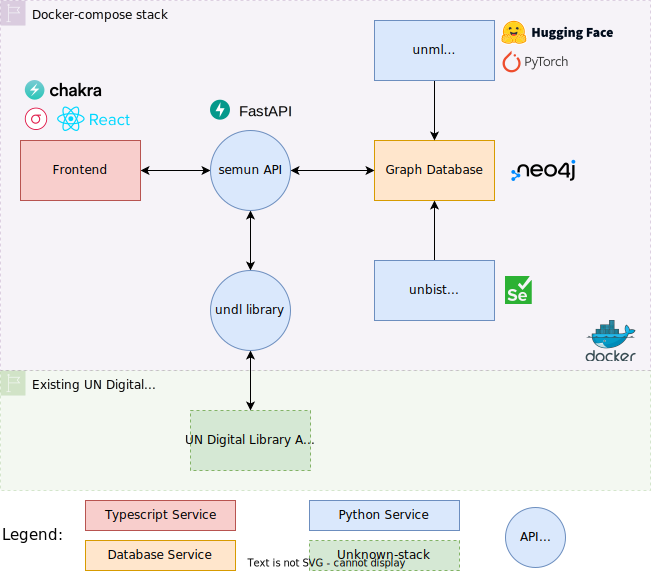
\includegraphics[width=\textwidth]{res/architecture-final.pdf}
    % \includegraphics*[width=0.8\textwidth]{res/architecture-final.png}
    \caption{Final stack architecture}
    % change caption position to the bottom

    \label{fig:architecture}
\end{figure}

\section{Final architecture} \label{sec:final-architecture}

The final architecture is a full-stack architecture, from the database to the frontend, handed in as a Docker compose stack: \repo{un-semun}.

The project consists of $7$ \faGithub{} GitHub repos:

\begin{itemize}
    \item \repo{un-semun}: The main repository with the \texttt{docker-compose} stack declaration.
    \item \repo{un-semun-frontend}: The frontend.
    \item \repo{un-semun-api}: The API for the frontend.
    \item \repo{undl}: The code for \texttt{undl}, a Python wrapper around the UN Digital Library API.
    \item \repo{un-unbis-thesaurus-scraper}: A scraper for the UNBIS Thesaurus taxonomy website.
    \item \repo{un-ml-pipeline}: Machine learning pipeline for UNDL documents.
    \item \repo{un-semun-misc}: Diverse scripts used for the project.
    \item \repo{un-semun-paper}: The code for this paper.
\end{itemize}

This paper will go through each of them in detail except for the paper repository.



\subsection{\texttt{un-semun-frontend}: A React \& Sigma.js frontend} \label{ssec:un-semun-frontend-a-react-sigma-js-frontend}

I used React combined with Typescript for the UI framework, as well as \href{https://chakra-ui.com/}{Chakra UI} for the UI components and \href{https://www.sigmajs.org/}{\texttt{Sigma.js}} via its React adapter \href{https://sim51.github.io/react-sigma/}{\texttt{@react-sigma}} for the network map. \href{https://graphology.github.io/}{\texttt{graphology}} was also used for graph manipulation in the frontend, mostly to iterate over graph elements to perform styling. The code is available here: \href{https://github.com/ClementSicard/un-semun-frontend}{\faGithub{} \texttt{un-semun-frontend}}.


\begin{figure}[!htb]
    \centering

    \includegraphics[width=\textwidth]{res/ml-pipeline.pdf}
    \caption{\texttt{un-semun-frontend} library: a dockerized machine learning pipeline for NER \& summarization}
    % change caption position to the bottom

    \label{fig:frontend-screenshot}
\end{figure}


The frontend was the part I was the least familiar with, but Chakra UI allowed to insert nice-looking components that I could customize based on my use case. It is composed in two panes:

\begin{itemize}
    \item \textbf{The search bar} (on top): the user can enter its prompt, which will be sent to the API (\ref{ssec:un-semun-api-an-api-for-un-semun-frontend-using-fastapi}) to retrieve the results.
    \item \textbf{The result list} (on the left). The results are displayed as a scrollable list of \texttt{Card} components, with the title, the summary, and the date of publication. The user can click on a card to display the document in the right pane.
    \item \textbf{The network map} (on the right). The results of the search are also displayed as a network map, with the documents, related United Nations bodies, topics from UNBIS Thesaurus taxonomy, and named entities extracted from the documents. The user can click on a node to display the document in the left pane. This map is also fetched using the API (\ref{ssec:un-semun-api-an-api-for-un-semun-frontend-using-fastapi}) and is based on the results of the machine learning pipeline (\ref{ssec:unml-the-machine-learning-pipeline}).
\end{itemize}




\subsection{\texttt{un-semun-api}: An API for \texttt{un-semun-front} using \texttt{FastAPI}} \label{ssec:un-semun-api-an-api-for-un-semun-front-using-fastapi}

The \texttt{un-semun-api} Python package was developed to provide an API for the frontend. It is a \href{https://fastapi.tiangolo.com/}{\texttt{FastAPI}} application, which is a Python framework for quickly and easily building APIs. It is a modern framework, which is fast, easy to use, and well documented. One nice feature is that it is also coupled with \href{https://docs.pydantic.dev/latest/}{\texttt{pydantic}} to perform data validation and serialization. This is very useful to ensure that the data sent to the frontend is valid, and to avoid having to write boilerplate code for (de)serialization.

This package mainly acts as a proxy between the frontend and the UNDL API through \repo{undl} library (\ref{ssec:undl-a-python-library-to-wrap-to-the-un-digital-library-api}), and is composed of $3$ main endpoints:

\begin{itemize}
    \item \texttt{/search}: This endpoint is used to perform a search query.  It takes a \texttt{GET} HTTP request with query parameter the prompt. Then, it uses \texttt{undl} (\ref{ssec:undl-a-python-library-to-wrap-to-the-un-digital-library-api}) library to perform the search on the UNDL API and returns the results to the frontend.

    \item \texttt{/graph}: This endpoint is used to get the graph corresponding to the above search query, also with an HTTP \texttt{GET} request with the prompt as unique query parameter. To optimize the process, it first gets the IDs of all documents returned by the search query on the given prompt, then it queries the Neo4j graph database (\ref{ssec:neo4j-graph-database}) to get the graph corresponding to these documents. Finally, it returns the graph to the frontend as \texttt{JSON} structured according to the format expected by the \href{https://graphology.github.io/}{\texttt{graphology}} Typescript library, which is used to model a graph and manipulate it as a programmatic object.

    \item \texttt{/query}: This endpoint creates a JSON with the response of both methods. It has been created to be directly queries by the frontend, and to obtain both the search results and the graph to display in a single HTTP request. It is actually the only one used in the latest version of the frontend.
\end{itemize}

Note that the API is dockerized and that it offers a basic in-memory query caching mechanism to avoid querying the UNDL API too often. This is done using a simple Python \texttt{dict} object in memory, which is not ideal but enough for the scope of this project.

\subsection{\texttt{undl}: A Python library to wrap to the UN Digital Library API} \label{ssec:undl-a-python-library-to-wrap-to-the-un-digital-library-api}

For the \texttt{undl} library, I used Python 3.10 with packages, with \texttt{requests} for the HTTP requests, \texttt{pandas} for the data manipulation, and \texttt{pydantic} for the data validation.

Its purpose is to query the UN Digital Library API, and to return the results in a structured way and convenient way. It converts the \texttt{MARCXML} response from the API to a \texttt{JSON} object and implements caching to save the results of the queries, and to avoid querying the API again if the same query is made. The client offers these main methods:

\begin{itemize}
    \item \texttt{query(...)}:
          Takes the prompt (e.g., \texttt{"Women in peacekeeping"}) as an argument, and returns the detailed results of the query as a \texttt{JSON} object. The API response is a list of detailed documents (the fields we actually collect are precised in \ref{ssec:neo4j-graph-database} for the \texttt{Document} node type).
          The main difference with a direct call to the UNDL API is that it converts the output to a \texttt{JSON} object. It is used by \repo{un-semun-api} (\ref{ssec:un-semun-api-an-api-for-un-semun-frontend-using-fastapi}).

    \item \texttt{getAllRecordIds(...)}:
          Same as \texttt{query}, but returns only the IDs of the documents, not their entire fields - hence is much faster. It is used by \repo{un-semun-api} (\ref{ssec:un-semun-api-an-api-for-un-semun-frontend-using-fastapi}) and \repo{un-ml-pipeline} (\ref{ssec:un-ml-pipeline-the-machine-learning-pipeline}).

    \item \texttt{queryBdId(...)}:
          Queries the API for a single document, given its \texttt{id}. It is used by \repo{un-ml-pipeline} (\ref{ssec:un-ml-pipeline-the-machine-learning-pipeline}).
\end{itemize}

These methods are callable either from the command-line interface (CLI), or from another Python script when imported as a library (see an example in Figure \ref{fig:undl-py})

\begin{figure}[!ht]
    \centering
    \includegraphics[width=0.6\textwidth]{res/import-undl.png}
    \caption{Querying the UNDL API from a Python script using \texttt{undl} library}
    \label{fig:undl-py}
\end{figure}

Note that \texttt{undl} requires a valid UNDL API key to work (set using the environment variable \texttt{UN\_API}), because the API calls are authenticated by this $36$ characters long key.



% UNBIST
\subsection{\texttt{un-unbis-thesaurus-scraper}: the UNBIS Thesaurus scraper} \label{ssec:un-unbis-thesaurus-scraper-the-unbis-thesaurus-scraper}

\subsubsection*{Tech stack of \texttt{un-unbis-thesaurus-scraper}} \label{sssec:tech-stack-of-un-unbis-thesaurus-scraper}




% unml
\subsection{\texttt{unml}: The machine learning pipeline} \label{ssec:unml-the-machine-learning-pipeline}

\begin{figure}[!htb]
    \centering

    \includegraphics[width=\textwidth]{res/ml-pipeline.pdf}
    \caption{\texttt{unml} library: a dockerized machine learning pipeline for NER \& summarization}
    % change caption position to the bottom

    \label{fig:ml-pipeline}
\end{figure}

\subsubsection*{Tech stack of \texttt{un-ml-pipeline}} \label{sssec:tech-stack-of-un-ml-pipeline}

\subsubsection{Parts} \label{sssec:parts}

\todo[inline]{Parts}

\subsubsection{Models} \label{sssec:models}
\todo[inline]{Models}

\subsubsection{API} \label{sssec:api}
\todo[inline]{API}
\todo[inline]{Connection to Neo4j}



\pagebreak
\subsection{Neo4j graph database} \label{ssec:neo4j-graph-database}

A graph database seemed to be the best choice to store the data extracted from the documents and the links between them, since it captures this relationship property and is able to retrieve it very efficiently. \href{https://neo4j.com/}{\texttt{Neo4j}} seemed to be the most accessible one to use, but other solutions exist (such as ArangoDB\footnote{\url{https://www.arangodb.com/}} or OrientDB\footnote{\url{https://orientdb.org/}}).

Here is the chosen data model for this project:

\subsubsection{Types of nodes} \label{sssec:types-of-nodes}

\begin{itemize}
      \item \texttt{Document}:
            This node type represents a document in the UNDL. It contains the document's \texttt{id} from the library management system, its summary (created when the document was run through the machine learning pipeline), symbol (some internal UN classification for the document - for instance \texttt{A/C.5/43/SR.50}), publication date, title, URL, and publication location.

      \item \texttt{Topic}:
            This node type represents a topic in the sense of the UNBIS Thesaurus taxonomy. I made a scraper \repo{un-unbis-thesaurus-scraper} (\ref{ssec:un-unbis-thesaurus-scraper-the-unbis-thesaurus-scraper}), and used it to retrieve all the topics from the taxonomy website, and inserted them into the database instance. Each topic has \texttt{name}, \texttt{cluster}, \texttt{id} fields, as well as label fields for each of the $6$ official UN languages (\texttt{labelEn}, \texttt{labelFr}, \texttt{labelEs}, \texttt{labelAr}, \texttt{labelZh}, \texttt{labelRu}).

      \item \texttt{MetaTopic}:
            UNBIS Thesaurus is structured as a hierarchy, and a \texttt{MetaTopic} is one of the top-level topics in this hierarchy. It has the same fields as a \texttt{Topic} node, and there are $18$ of them.\footnote{\href{https://metadata.un.org/thesaurus/?lang=en}{The list of \texttt{MetaTopic} nodes from UNBIS Thesaurus website}}

      \item \texttt{Country}:
            This node type represents a country as a member state of the UN. It has the same fields as a \texttt{Topic} node, and there are $193$ of them.\footnote{\href{https://www.un.org/en/about-us/member-states}{The list of the $193$ UN member states from the UN website}} The data to create these nodes was retrieved from the UN website, and the Cypher queries were generated using a Python script in \repo{un-semun-misc} (\ref{ssec:un-semun-misc}).

      \item \texttt{UNBody}:
            This node type represents a body of the United Nations. A body of the UN is an organizational unit within the United Nations system, established to carry out specific functions ranging from peacekeeping and humanitarian aid to diplomatic negotiations and policy recommendations. Some famous examples include the Security Council, the World Health Organization (WHO), the International Monetary Fund (IMF) etc... As for the countries, the data was retrieved from the UN website, and the Cypher queries were generated using a Python script in \repo{un-semun-misc} (\ref{ssec:un-semun-misc}).


\end{itemize}

\subsubsection{Types of relationships} \label{sssec:types-of-relationships}

These nodes are linked together by the following relationships:

\begin{itemize}
      \item \texttt{-[REFERENCES]->}:
            This relationship type links a \texttt{Document} node to a \texttt{Country} or \texttt{Entity} node, and is self-explanatory: the document references the target entity. This relationship is extracted by the machine learning pipeline.

      \item \texttt{-[HAS\_SUBTOPIC]->}:
            Links a \texttt{MetaTopic} node to a \texttt{Topic} node to explicit the hierarchy between the two nodes. It was created by the scraper.

      \item \texttt{-[IS\_ABOUT]->}:
            Links a \texttt{Document} node to a \texttt{Topic} node to indicate that the \texttt{Document} has been classified by UN Digital Library staff as a document about the \texttt{Topic}. This relationship is extracted from the UNDL API response.

      \item \texttt{-[RELATED\_TO]->}:
            Links a \texttt{Topic} node to another \texttt{Topic} node indicate a semantic link between the two topics. This relationship is extracted from the UNBIS Thesaurus website, using the scraper as well.

\end{itemize}



\subsection{\texttt{un-semun}: The main repository} \label{ssec:un-semun-the-main-repository}

\texttt{un-semun} is a repository that englobes all other repositories as submodules. It also contains the \texttt{docker-compose} stack declaration, which points to Dockerfiles in submodules. They are updated using the \texttt{Makefile} when new commits are added to the submodules. The port forwardings and environment variables are also declared here. This is the main entry point to run the whole stack.




\subsection{\texttt{un-semun-misc}} \label{ssec:un-semun-misc}







\subsection{General tech stack notes} \label{ssec:general-tech-stack-notes}

All the services composing of the stack are dockerized (i.e., they live in their own Docker container but their storage and network interface can be shared), and they are orchestrated and connected using \texttt{docker-compose}\footnote{\url{https://docs.docker.com/compose/}}.

For all the Python components in the stack (the blue components in Figure \ref{fig:architecture}), the dependencies are managed using \texttt{poetry}\footnote{\url{https://github.com/python-poetry/poetry}}.
